\chapter{Inéquations de degré $\geq 2$}

Dans ce chapitre, nous étudierons des inéquations. Il est donc important d'être au clair sur la notion d'intervalle, ainsi que sur le signe des fonctions affines et quadratiques. On rappelle ici l'essentiel :

\vspace{5mm}

\shadowbox{
\begin{minipage}{0.9\textwidth}
\begin{itemize}
\item Pour la fonction affine $f(x) = ax+b$, le signe de $a$ est placé sous $+\infty$. La fonction change de signe au zéro.
\item Pour la fonction quadratique $f(x) = ax^2 + bx + c$, le signe de la fonction est le signe de $a$ sauf entre les zéros.
\end{itemize}
\end{minipage}
}

\vspace{5mm}

Rappelons également qu'il est difficile, sans graphique, de déterminer les solutions d'une inéquation qui compare deux fonctions. Aussi pour toutes ces inéquations, on préfère commencer par placer tous les termes du même côté de l'inéquation, en se rappelant que si l'on multiplie ou divise par un terme négatif, il faut changer le sens de l'inéquation.

\section{Inéquations du deuxième degré}

Comme rappelé en préambule, il faut commencer par placer tous les termes du même côté, puis déterminer les zéros de fonction. On peut ensuite faire le tableau des signes du polynôme et déterminer graphiquement, puis sous forme d'intervalle, la solution de l'inéquation.

\begin{exemple}
Résoudre l'inéquation :
$$
x^2 -3x +3 \geq 3x-2
$$
On commence par placer tous les termes du même côté :
$$
x^2 -6x +5 \geq 0
$$
Ensuite on trouve les deux racines du polynôme non nul :
$$
x_1 = 1 \mbox{ et } x_2 = 5
$$
et on détermine les signes du polynôme :
$$
\begin{array}{l|l|l|l|l|l|l|l}
x & -\infty &  & 1 & & 5 & & +\infty\\
\hline
x^2-6x+5 & + & + & 0 & - & 0 & + & + 
\end{array}
$$
Puisqu'on doit trouver quand le polynôme est plus grand que zéro ($\geq 0$), les solutions sont les valeurs qui donnent un résultat positif ($+$). Ainsi 
$$
S=]-\infty ; 1] \cup [5;+\infty[
$$
\end{exemple}

\section{Inéquations fractionnaires}\index{Inéquation!fractionnaire}

Attention à toujours commencer par placer tous les termes du même côté, sous une seule fraction. Il peut donc être utile de revoir le thème lié aux opérations sur les fractions.

Pour résoudre une inéquation fractionnaire, il va falloir déterminer le signe de la fraction en fonction des valeurs de $x$. Or ces signes dépendent de ceux du numérateur et du dénominateur. Aussi on va étudier séparément les signes du dénominateur et du numérateur, puis assembler ces deux tableaux pour déterminer les signes de la fraction.

Les règles des signes sont les mêmes que pour les multiplications, mais il faut avoir une attention particulière pour les zéros du dénominateur qui ne peuvent pas faire partie de la solution. Ainsi pour un zéro au dénominateur, on va placer deux barres verticales sous le signe de la fraction ($||$).

\begin{exemple}
Résoudre l'inéquation 
$$
\frac{x^2 - 5x + 6}{x-2} < 0
$$
Commençons par déterminer les racines des polynômes numérateur et dénominateur :
$$
x^2 - 5x + 6 = 0 \ssi x_1 = 2 \mbox{ et } x_2 = 3
$$
et 
$$
x-2 = 0 \ssi x = 2
$$
On peut passer au tableau des signes de la fraction :
$$
\begin{array}{l l|l|l|l|l|l|l|l}
&x& -\infty & & 2 & & 3 & & +\infty\\
\hline
\hline
\mbox{numérateur }&x^2 -5x + 6 & + & + & 0 & - & 0 & + & +\\
\hline
\mbox{dénominateur }&x-2 &- & - & 0 & + & + & + & + \\
\hline 
\hline
\mbox{fraction }&\frac{x^2 - 5x + 6}{x-2} & - & - & || & - & 0 & + & + \\
\end{array}
$$
Comme nous cherchons les valeurs de $x$ qui rendent la fraction négative ($<0$), la solution est donnée par les $-$ de la dernière ligne :
$$
S= ]-\infty ; 2[
$$
\end{exemple}

\section{Inéquation de degré supérieur à $2$}\index{Inéquation!produit}

Une fois tous les termes du même côté et le polynôme réduit, si le degré de ce dernier est toujours supérieur à $2$, il va falloir le factoriser pour étudier séparément les signes de chaque facteur, puis assembler les tableaux, comme pour les fractions, afin de connaître les signes du produit.

Cette fois cependant, puisqu'il n'y a pas de dénominateur, il n'y a pas besoin de porter une attention particulière aux zéros que l'on peut rencontrer.

\begin{exemple}
Factoriser 
$$
x^3 -2x^2 + x \leq 0
$$
On commence par factoriser le polynôme  afin de n'avoir que des polynômes de degré $\leq 2$, par exemple par une mise en évidence
$$
x\cdot (x^2 - 2x + 1) \leq 0
$$
On détermine les racines des deux polynômes :
$$
x = 0 \ssi x = 0
$$
et 
$$
x^2 -2x + 1 = 0 \ssi x_1 = x_2 = 1 \, (\Delta = 0)
$$
On a donc le tableau suivant :
$$
\begin{array}{l l|l|l|l|l|l|l|l}
&x& -\infty & & 0 & & 1 & & +\infty\\
\hline
\hline
\mbox{premier facteur }&x & - & - & 0 & + & + & + & +\\
\hline
\mbox{deuxième facteur }&x^2 - 2x + 1 &+ & + & + & + & 0 & + & + \\
\hline 
\hline
\mbox{produit }&x\cdot(x^2 -2x+1) & - & - & 0 & + & 0 & + & + \\
\end{array}
$$
Comme nous cherchons les valeurs de $x$ qui rendent le produit négatif ou nul ($\leq 0$), la solution est donnée par les $-$ et les $0$ :
$$
S=]-\infty;0] \cup \{1\}
$$
\end{exemple}

\section{Système d'inéquations}

Comme pour les système d'inéquations du premier degré, on commence par résoudre chaque inéquation de manière individuelle, comme expliqué plus haut. On compare ensuite les solutions graphiques pour déterminer l'intersection de ces dernières.

\begin{exemple}
Résoudre le système 
$$
\left\{
\begin{array}{rcl}
2-3x &\geq& 0\\
x^2 + 3x -4 &<& 0\\
\frac{1}{x} &\geq & 0
\end{array}
\right.
$$
Par les méthodes précédentes, on trouve \textcolor{red}{(Attention à ne pas tout mettre dans un seul tableau !)} :
$$
\begin{array}{l|l|l|l|l|l}
x & -\infty & & \frac{2}{3} &  & +\infty\\
\hline
2-3x & + & + & 0 & - & - \\
\end{array}
$$

$$
\begin{array}{l|l|l|l|l|l|l|l}
x & -\infty &  & -4 & & 1 & & +\infty\\
\hline
x^2 + 3x -4 & + & + & 0 & - & 0 & + & +\
\end{array}
$$

$$
\begin{array}{l|l|l|l|l|l}
x & -\infty & & 0 & & +\infty \\
\hline
1 & + & + & + & + & + \\
\hline
x & - & - & 0 & + & + \\
\hline
\hline
\frac{1}{x} & 0 & - & || & + & 0\\
\end{array}
$$
Puis on dessine sous voie graphique les solutions :
\begin{center}
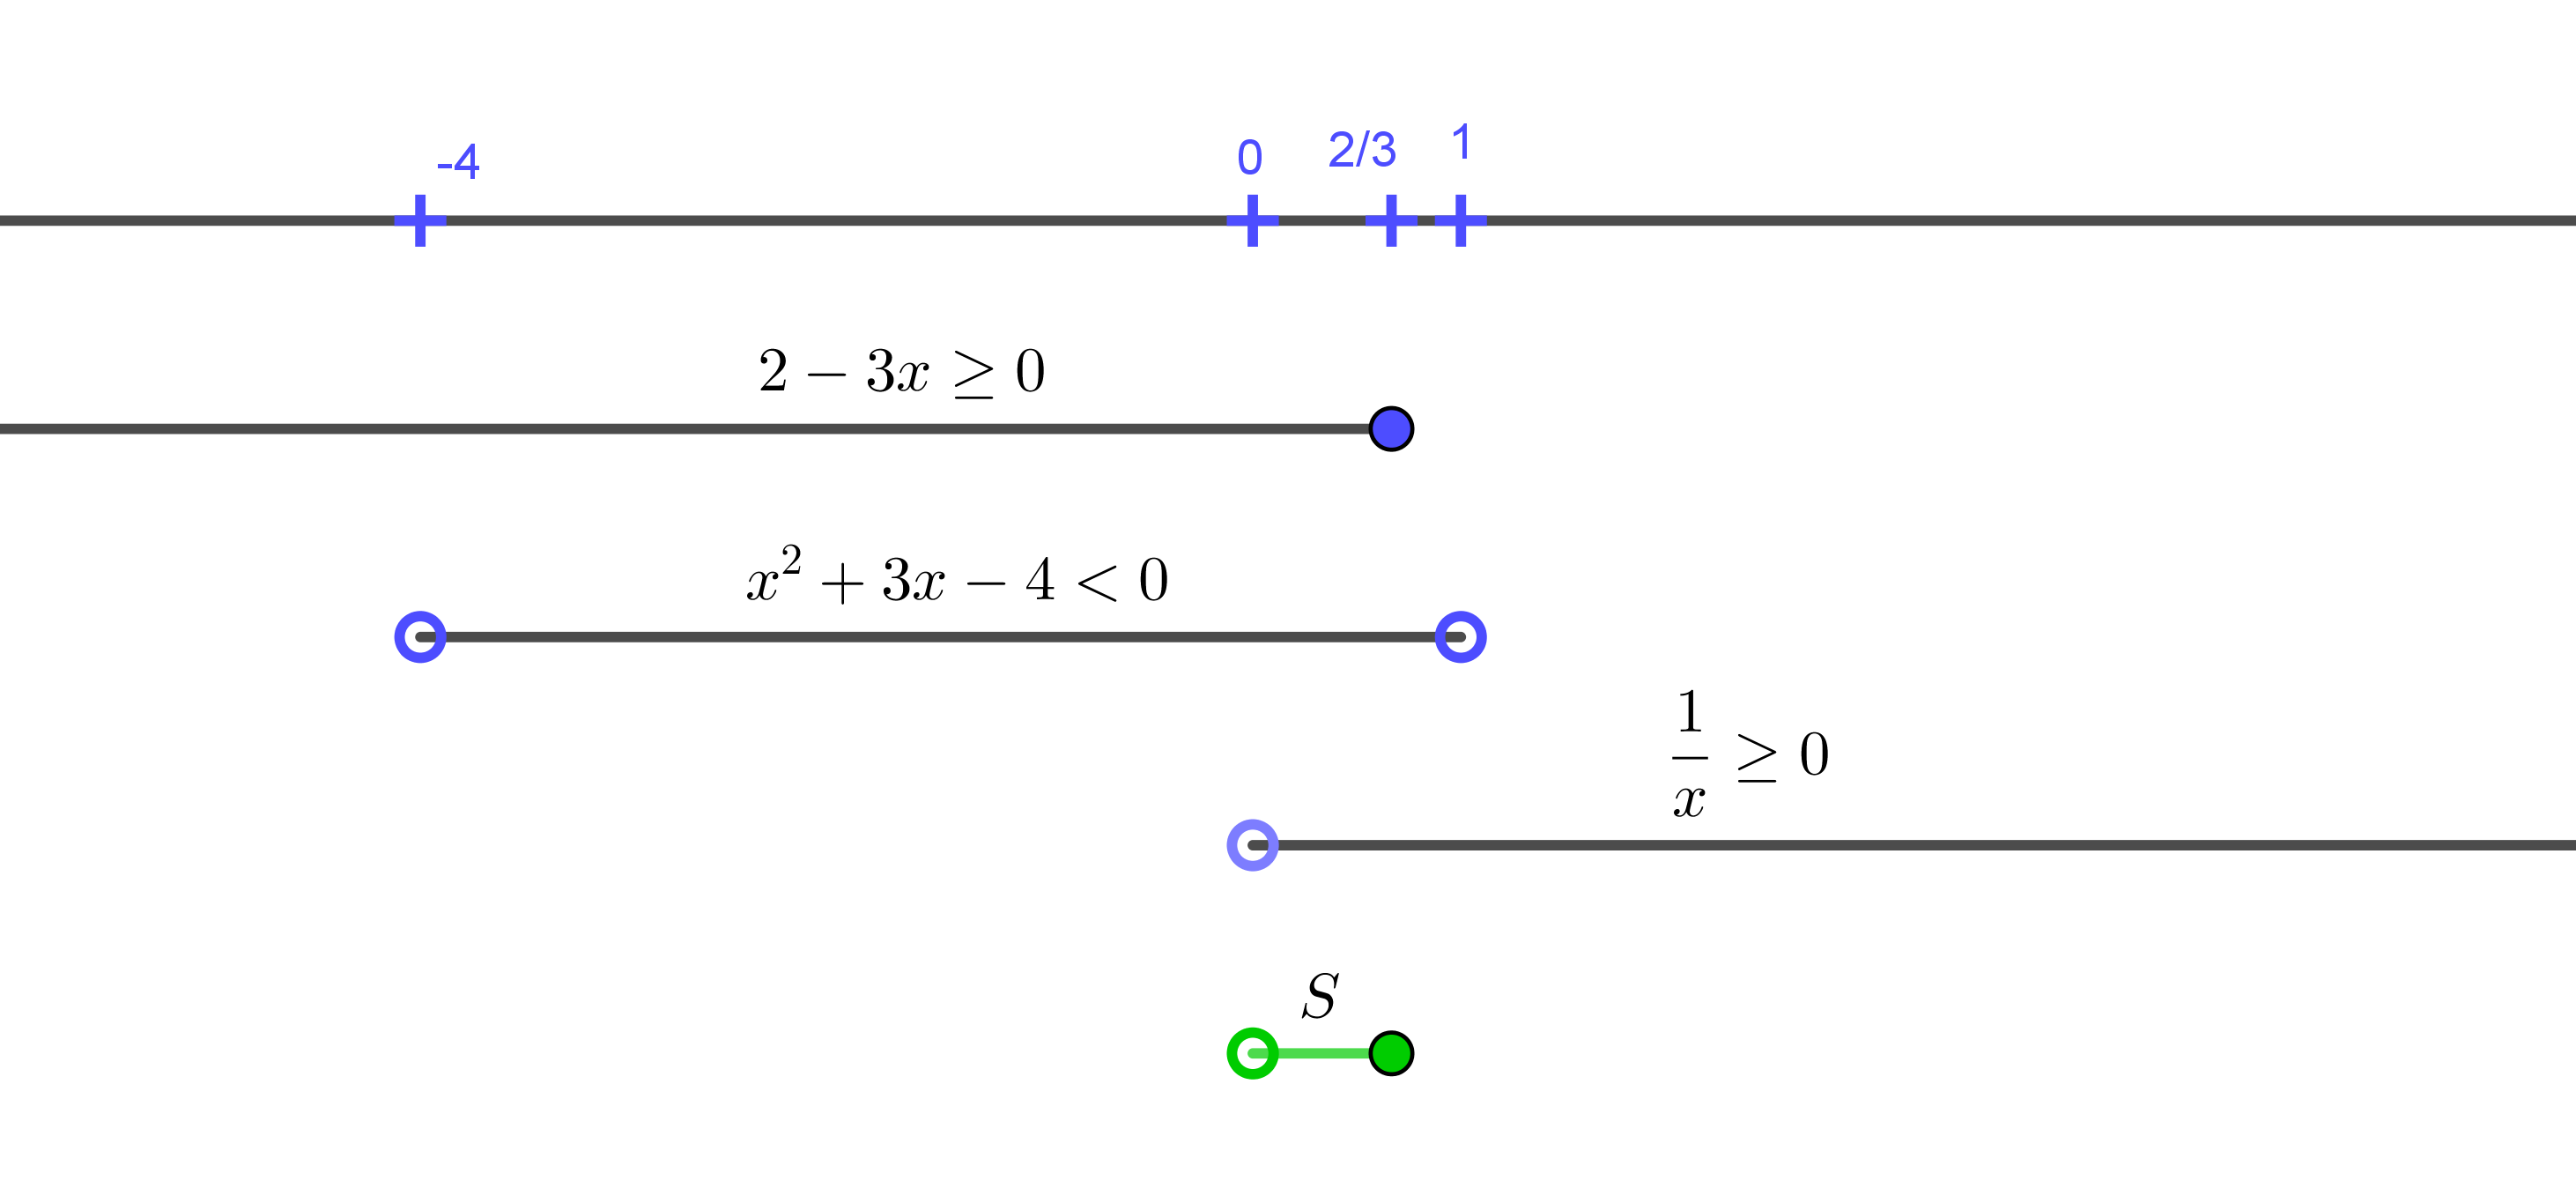
\includegraphics[width = 0.9 \textwidth]{inequation2/systeme.png}
\end{center}
La solution est donc donnée par
$$
S=\left]0;\frac{2}{3}\right]
$$
\end{exemple}

\section{Exercices}

\begin{exercice}
Résoudre les inéquations suivantes :
\begin{multicols}{2}
\begin{enumerate}
\item ${{x}^{2}}+2x-15>0$ 
\item ${{x}^{2}}-5x+4<0$ 
\item $-2{{x}^{2}}+3x+2>0$ 
\item $-3{{x}^{2}}+7x-2\le 0$ 
\item $x{}^{2}+31x+150>0$ 
\item ${{x}^{2}}-10\ge 3x$
\item $-{{x}^{2}}-7>x-19$
\item ${{x}^{2}}+7>3x$
\item ${{x}^{2}}\ge 7x-8$
\item ${{x}^{2}}\ge 16$
\item ${{x}^{2}}<6x$
\item $256<{{x}^{2}}$
\item $x(x-2)<6x$
\item $3x(x-3)\le 5\left( x-3 \right)$
\item $\left( 2-x \right)\left( 4x-5 \right)\ge 0$
\end{enumerate}
\end{multicols}
\end{exercice}

\begin{exercice}
Résoudre les inéquations rationnelles suivantes :
\begin{multicols}{2}
\begin{enumerate}
\item $\frac{x+2}{x-3}>0$ 
\item $\frac{-x+5}{5+x}\le 0$ 
\item $\frac{3x-1}{3-x}\ge 0$ 
\item $\frac{1}{4{{x}^{2}}-x-3}\le 0$ 
\item $\frac{2x+1}{3-x}\ge -1$
\item $\frac{x}{2x+3}\le \frac{1}{2}$
\item $\frac{2}{2x-3}\ge \frac{1}{x}$
\item $\frac{{{x}^{2}}-4}{{{x}^{2}}-2x-3}\le 0$
\item $\frac{x-1}{{{x}^{2}}-2x-8}>0$
\item $\frac{{{x}^{3}}-5{{x}^{2}}+6x}{{{x}^{2}}-2x+1}\ge 0$
\item $\frac{{{x}^{3}}-2{{x}^{2}}+x}{{{x}^{2}}-1}\le 0$
\item $\frac{{{x}^{4}}-81}{-{{x}^{3}}-{{x}^{2}}-x}\le 0$
\end{enumerate}
\end{multicols}
\end{exercice}

\begin{exercice}
Résoudre les systèmes suivants :
\begin{multicols}{2}
\begin{enumerate}
\item $\left\{ \begin{array}{ll}
  & 12{{x}^{2}}-5x-2>0 \\ 
 & 12{{x}^{2}}+5x+38>0 \\ 
 & 24{{x}^{2}}-67x+38>0 \\ 
\end{array}{ll} \right.$
\item $\left\{ \begin{array}{ll}
  & {{x}^{2}}-2x-8\ge 0 \\ 
 & -\frac{x-3}{2x-4}<0 \\ 
 & x+5\ge -3 \\ 
\end{array}{ll} \right.$

\item $\left\{ \begin{array}{ll}
  & {{x}^{2}}\le 9 \\ 
 & {{x}^{2}}-16\ge 4\left( x-4 \right) \\ 
\end{array}{ll} \right.$

\item $\left\{ \begin{array}{ll}
  & \frac{x\left( {{x}^{2}}-5x+6 \right)}{{{\left( x-1 \right)}^{2}}}\ge 0 \\ 
 & -x-1<0 \\ 
 & \frac{2x-1}{2x-3}\ge 0 \\ 
\end{array}{ll} \right.$
\item $\left\{ \begin{array}{ll}
  & 2{{x}^{2}}-5x-3\ge 0 \\ 
 & {{x}^{2}}-3x-4\le 0 \\ 
 & {{x}^{2}}-1>0 \\ 
\end{array}{ll} \right.$
\item $\left\{ \begin{array}{ll}
  & \frac{-5}{{{x}^{2}}-5x+6}<0 \\ 
 & -\frac{x-4}{-x-5}\ge 0 \\ 
 & \frac{-8x}{{{x}^{2}}+9}\ge 0 \\ 
\end{array}{ll} \right.$
\item $\left\{ \begin{array}{ll}
  & \frac{3x}{x-5}<\frac{4}{2x+6} \\ 
 & \frac{1}{2}{{x}^{2}}-x>\frac{x}{4} \\ 
 & 5x+20\ge 0 \\ 
\end{array}{ll} \right.$
\end{enumerate}
\end{multicols}
\end{exercice}


